\documentclass{article}
\usepackage[utf8]{inputenc}
\usepackage[backend=biber]{biblatex}
\usepackage{amssymb}
\usepackage{amsmath}
\usepackage{dsfont}
\addbibresource{bib.bib}
\setlength{\parindent}{0em}
\bibliography{bib}
\setlength{\parskip}{6pt}
\usepackage[margin=1.0in]{geometry}
\usepackage{graphicx}
\usepackage{caption}
\usepackage{subcaption}
\usepackage{wrapfig}
\usepackage{url}

\title{Intro to deep learning with PyTorch}
\author{Miguel A. Saavedra-Ruiz}
\date{May 2020}
\linespread{1.0}

\nocite{*}


\begin{document}

\maketitle

\section*{Recurrent neural networks}

To understand what recurrent neural networks (RNN) are and the difference between RNN and LSTM imagine the next example. Imagine a regular neural network which recognizes images and the image in Fig. \ref{fig:f1} is fitted in the network and the neural neural network guesses that the image is most likely a dog with a small chance of being a wolf and an even smaller chance of being a goldfish. However, what if the image is actually a wolf?


\begin{figure}[ht]
    \centering
    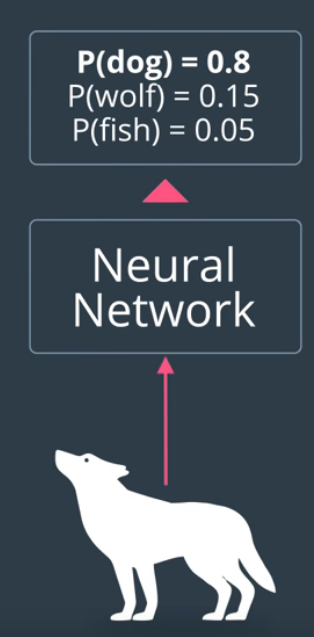
\includegraphics[width=0.25\textwidth,height=0.25\textheight,keepaspectratio]{images/fitting.png}
    \captionsetup{justification=centering}
    \caption{Fitting an image in a neural network}
    \label{fig:f1}
\end{figure}

To hint the algorithm about what animal it really is, let's say that the wolf appeared in a TV show about nature and the previous image before the wolf was a bear and the previous one was a fox. In this case, the idea is to use this information to hint the algorithm that the last image is a wolf and not a dog. Therefore, a good idea is to analyze each image with the same copy of a neural network. But, using the output of the neural network as a part of the input of the next one Fig. \ref{fig:f2}. 

\begin{figure}[ht]
    \centering
    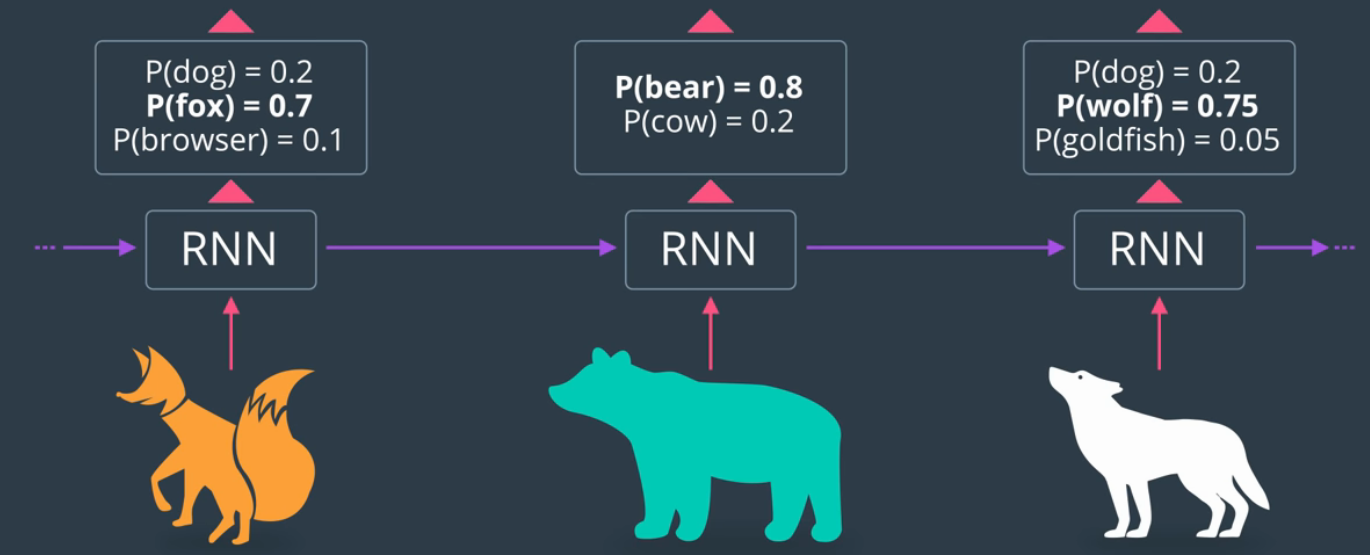
\includegraphics[width=0.5\textwidth,height=0.5\textheight,keepaspectratio]{images/recurrent.png}
    \captionsetup{justification=centering}
    \caption{Feeding a neural network with another neural networl}
    \label{fig:f2}
\end{figure}

This should improve the prediction results. Mathematically,it is just the combination of vectors in a linear function, which will then be squished with an activation function, which could be sigmoid or hyperbolic tan. This way the algorithm can use previous information and the final neural network will know that the show is about wild animals in the forest and actually use this information to correctly predict that the image is of a wolf and not a dog.

However, the last architecture has some drawbacks. Imagine that the bear appeared a while ago and the two recent images are a tree and a squirrel Fig. \ref{fig:f3}. Based on those two, it is hard to really know if the new image is a dog or a wolf. Since trees and squirrels are just as associated to domestic animals as they are with forest animals. The information about being in the forest comes all the way back from the bear. However, as it has been seen, information coming in gets repeatedly squished by sigmoid functions, training a network using backpropagation all the way back, will lead to problems such as the vanishing gradient problem. Hence by this point pretty much all the bear information has been lost. That's a problem with recurring neural networks; that the memory that is stored is normally short term memory.

\begin{figure}[ht]
    \centering
    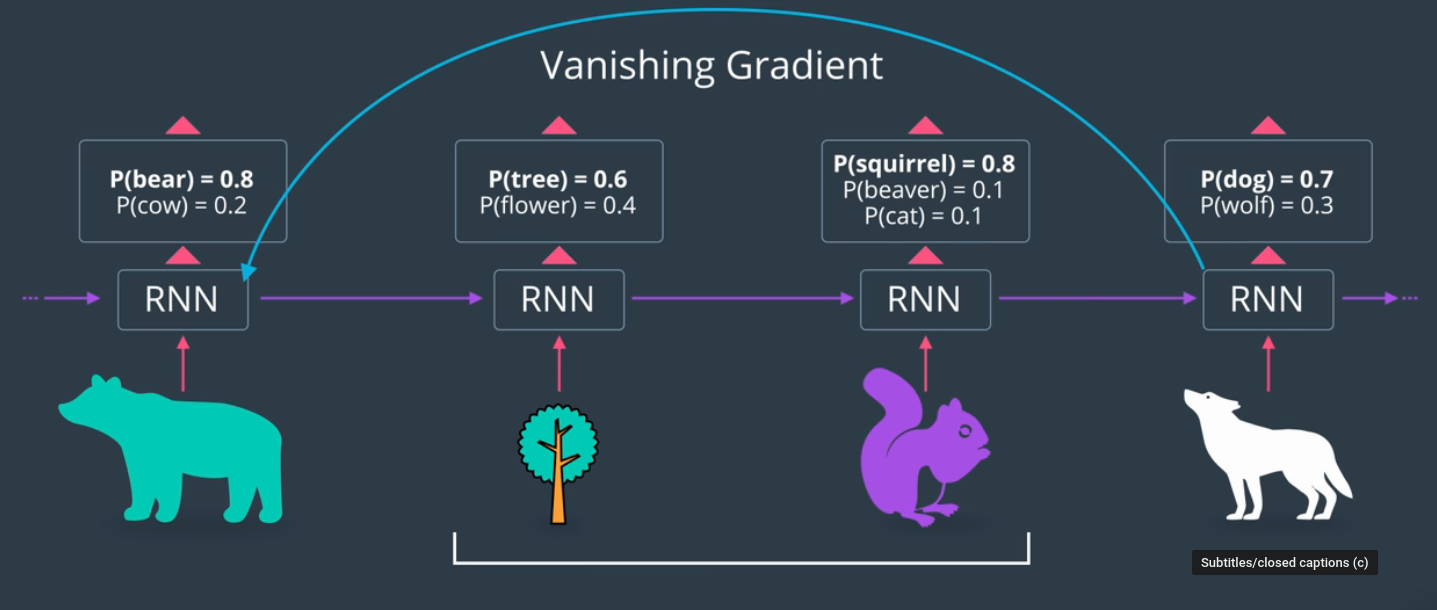
\includegraphics[width=0.65\textwidth,height=0.65\textheight,keepaspectratio]{images/drawback_rnn.png}
    \captionsetup{justification=centering}
    \caption{Drawbacks with RNN}
    \label{fig:f3}
\end{figure}

To solve the last problem, LSTMs or long short term memory networks are the solution to this issue. 
In summary, a RNN works as follows; memory comes in and merges with a current event and the output comes out as a prediction of what the input is and also, as part of the input for the next iteration of the neural network Fig. \ref{fig:f4}.

\begin{figure}[ht]
    \centering
    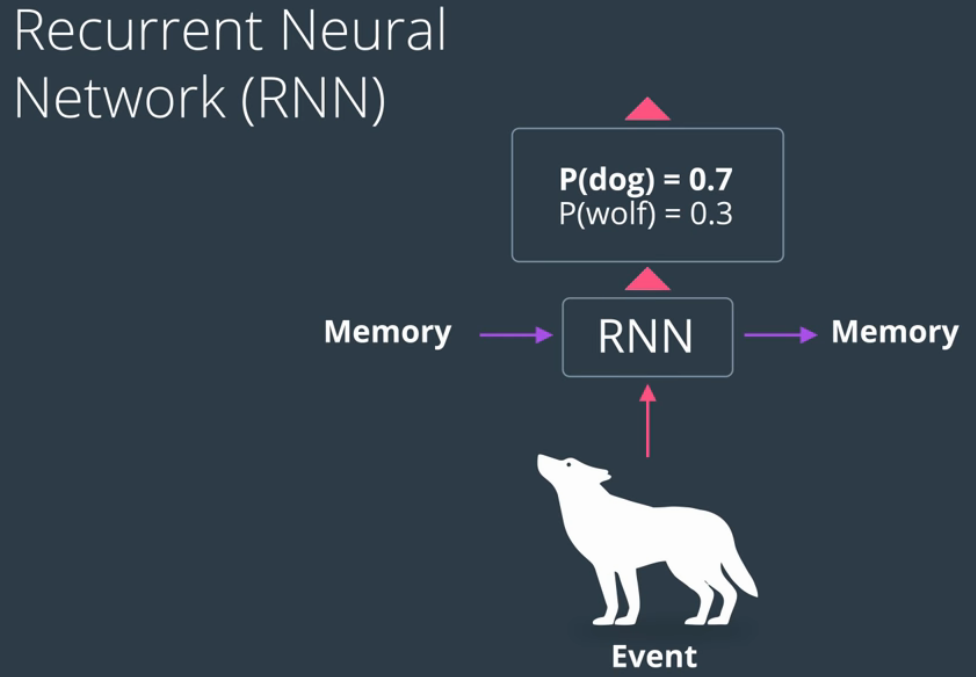
\includegraphics[width=0.45\textwidth,height=0.45\textheight,keepaspectratio]{images/rnn.png}
    \captionsetup{justification=centering}
    \caption{The general RNN architecture}
    \label{fig:f4}
\end{figure}

On the other hand, LSTM works as follows; it keeps track not just of memory but of long term memory, which comes in and comes out and also, short term memory, which also comes in and comes out Fig. \ref{fig:f5}. In every stage the long and short term memory in the event get merged. Therefore, a new long term memory, short term memory and a prediction are created. This architecture protects old information more.

\begin{figure}[ht]
    \centering
    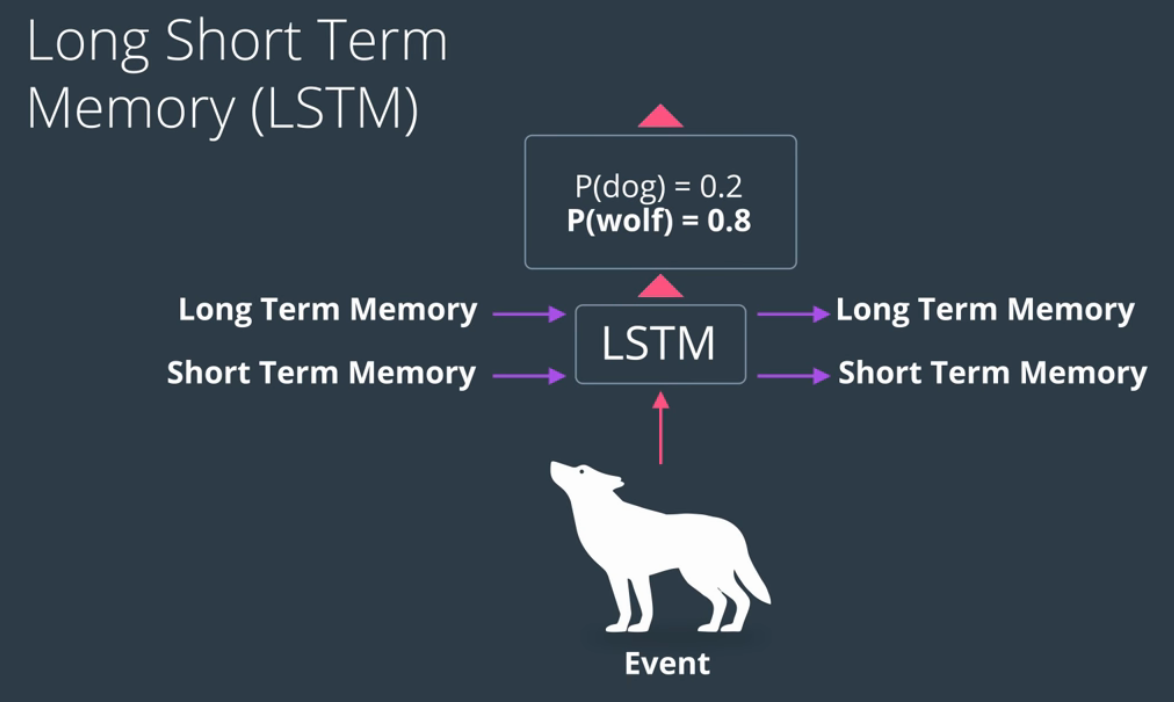
\includegraphics[width=0.55\textwidth,height=0.55\textheight,keepaspectratio]{images/lstm.png}
    \captionsetup{justification=centering}
    \caption{The general LSTM architecture}
    \label{fig:f5}
\end{figure}

The LSTM architecture can be described using the following example. 

Imagine the next example Fig. \ref{fig:f6} where the long term memory is represented by an elephant, the short term memory by a fish and the event will still be represented by a wolf.

\begin{figure}[ht]
    \centering
    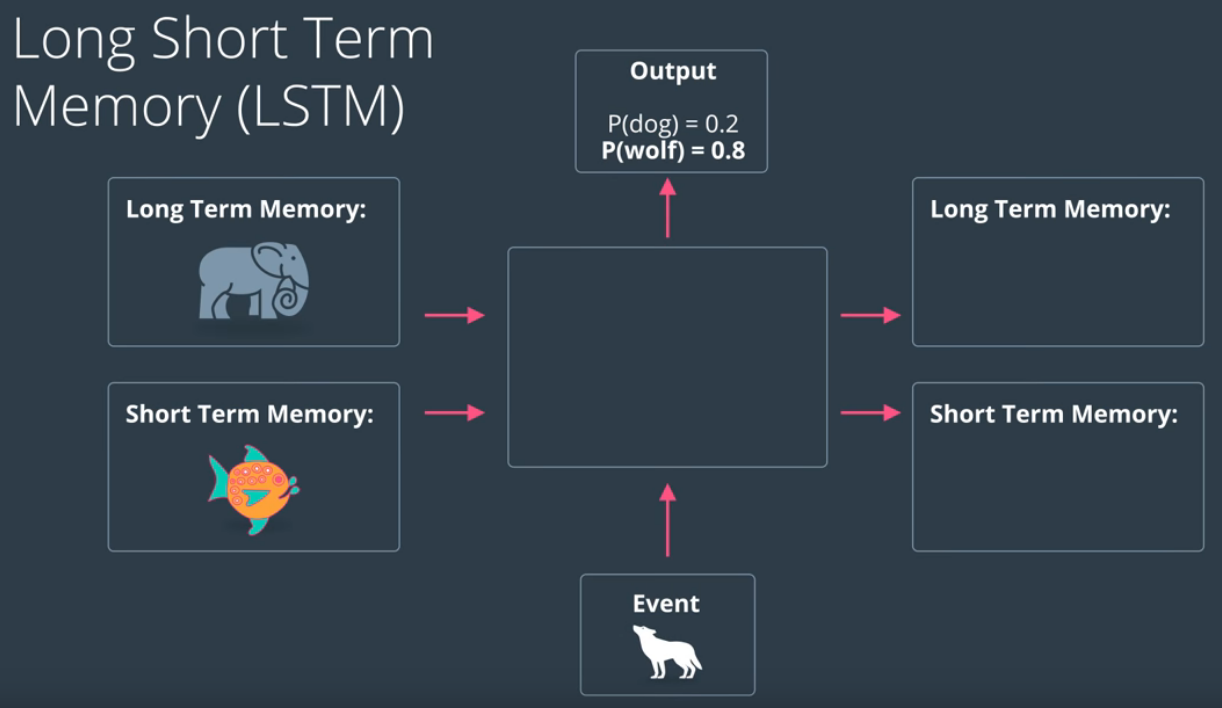
\includegraphics[width=0.7\textwidth,height=0.7\textheight,keepaspectratio]{images/lstm_example.png}
    \captionsetup{justification=centering}
    \caption{LSTM example}
    \label{fig:f6}
\end{figure}

So LSTM works as follows: the three pieces of information (Long term memory, short term memory and event Fig. \ref{fig:f6}) go inside the node some math happens inside which updates the output. These outputs are a long term memory, a short term memory and the prediction of the event. More specifically the architecture of the LSTM contains something called gates. It contains a forget gate, a learn gate, a remember gate, and a use gate Fig. \ref{fig:f7}.


\begin{figure}[ht]
    \centering
    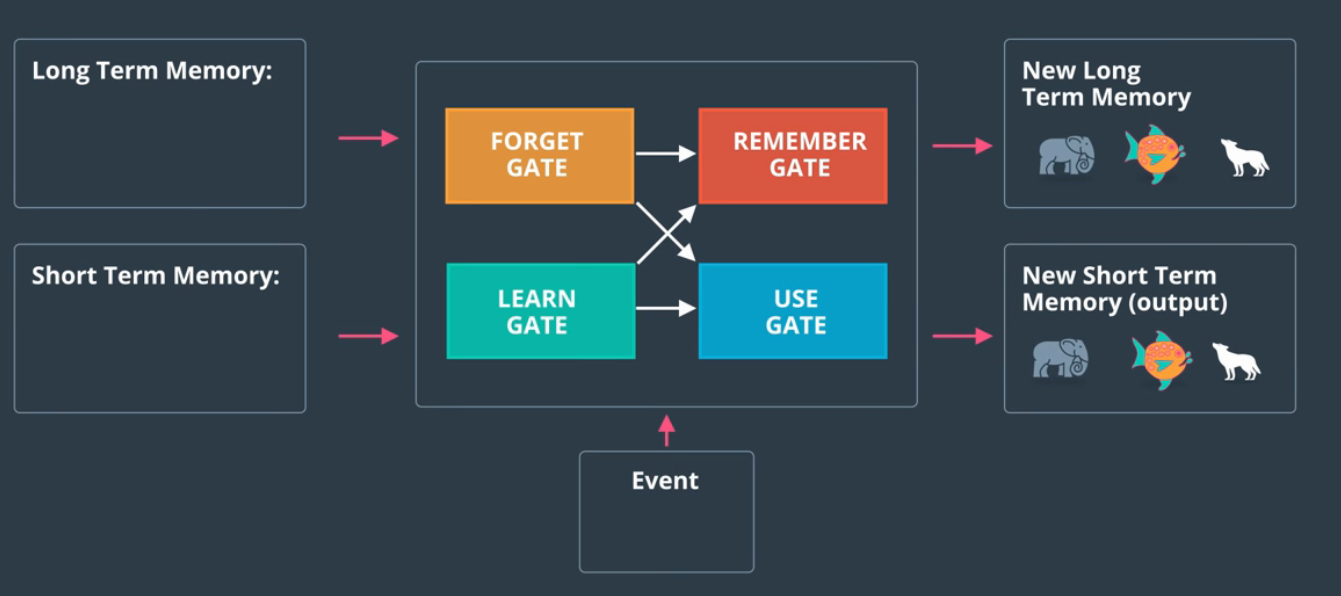
\includegraphics[width=0.7\textwidth,height=0.7\textheight,keepaspectratio]{images/lstm_example2.png}
    \captionsetup{justification=centering}
    \caption{LSTM gates}
    \label{fig:f7}
\end{figure}

The detailed explanation of how these gates work is as follows. The long term memory goes to the forget gate where it forgets everything that it doesn't consider useful. The short term memory and the event are joined together in the learn gate, containing the information that the LSTM recently learned and it removes any unnecessary information.

Subsequently, the long term memory that have not been forgotten yet (Forget gate) plus the new information that the node learned (Learn gate) get joined together in the remember gate. Since it's called remember gate, what it does is it outputs an updated long term memory. An example of what a long term memory looks like is seen in Fig. \ref{fig:f7} (this information will be remembered in the future). Finally, the use gate is the one that decides what information will be used from what was previously know plus what the node just learned to make a prediction. Taking both inputs from the long term memory and the short term memory will create new information and hence, create a new short term memory output. The output becomes both the prediction and the new short term memory.
 
Overall, the information from one LSTM cell moves towards another one and another one saving information from the past and propagating it towards the future to produce accurate predictions and keep information from the past Fig. \ref{fig:f8}. The long term memory is denoted as \textbf{LTM} and the short term memory as \textbf{STM}. It is important to note that the short term memory is the output or the prediction of the network.
 
\begin{figure}[ht]
    \centering
    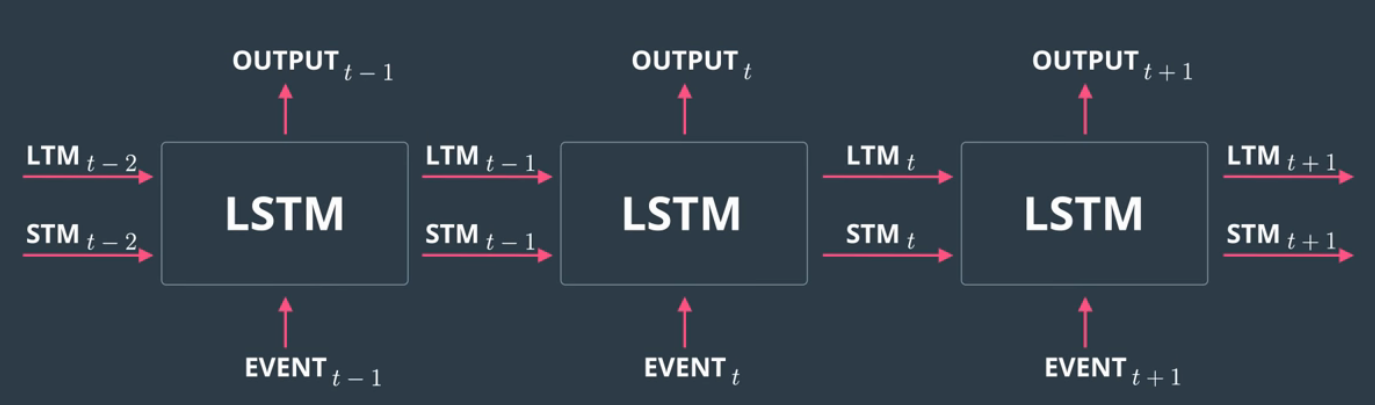
\includegraphics[width=0.7\textwidth,height=0.7\textheight,keepaspectratio]{images/lstm_nodes.png}
    \captionsetup{justification=centering}
    \caption{LSTM nodes connection}
    \label{fig:f8}
\end{figure}
 
To continue with the explanation of the math behind LSTM, let's first recall the architecture of a RNN Fig. \ref{fig:f9}. Basically what this network does is take the event \(E_t\) and memory \(M_{t-1}\), coming from the previous point in time and apply a simple tanh or sigmoid activation function to obtain the output and then the memory \(M_t\). Specifically, the network joins these two vectors and multiply them by a matrix \(W\) and add a bias \(b\). Finally the output is squished with the tanh function, and that gives us the output \(M_t\) Eq. \eqref{eq:1}.

\begin{figure}[ht]
    \centering
    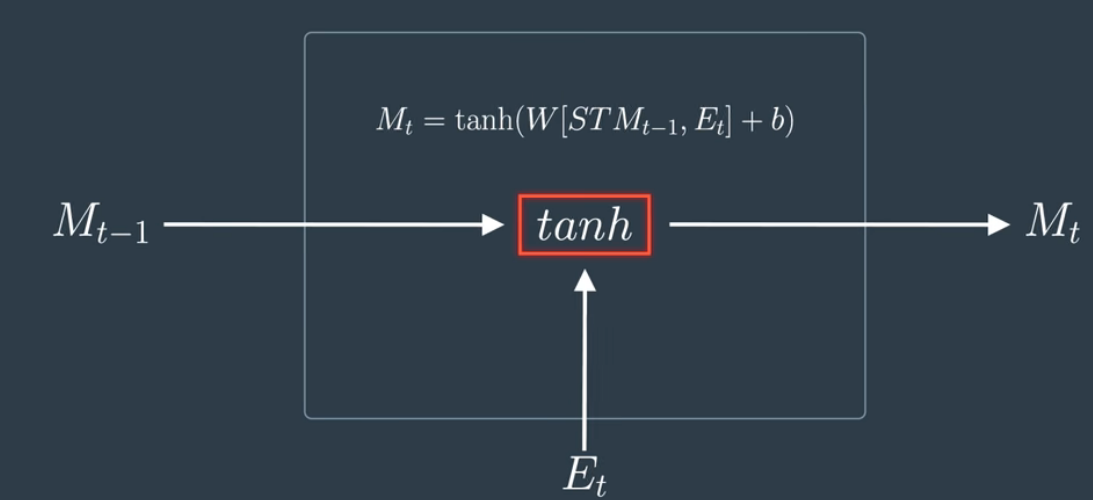
\includegraphics[width=0.5\textwidth,height=0.5\textheight,keepaspectratio]{images/recurrent_node.png}
    \captionsetup{justification=centering}
    \caption{Mathematical operation in a recurrent node}
    \label{fig:f9}
\end{figure}


\begin{equation}
M_t = tanh(W[ST M_{t-1}, E_t] + b)
\label{eq:1}
\end{equation}

The LSTM architecture is very similar to the recurrent neural network's architecture, except with more nodes inside and with two inputs and outputs since it keeps track of the long- and short-term memories Fig. \ref{fig:f10}.

\begin{figure}[ht]
    \centering
    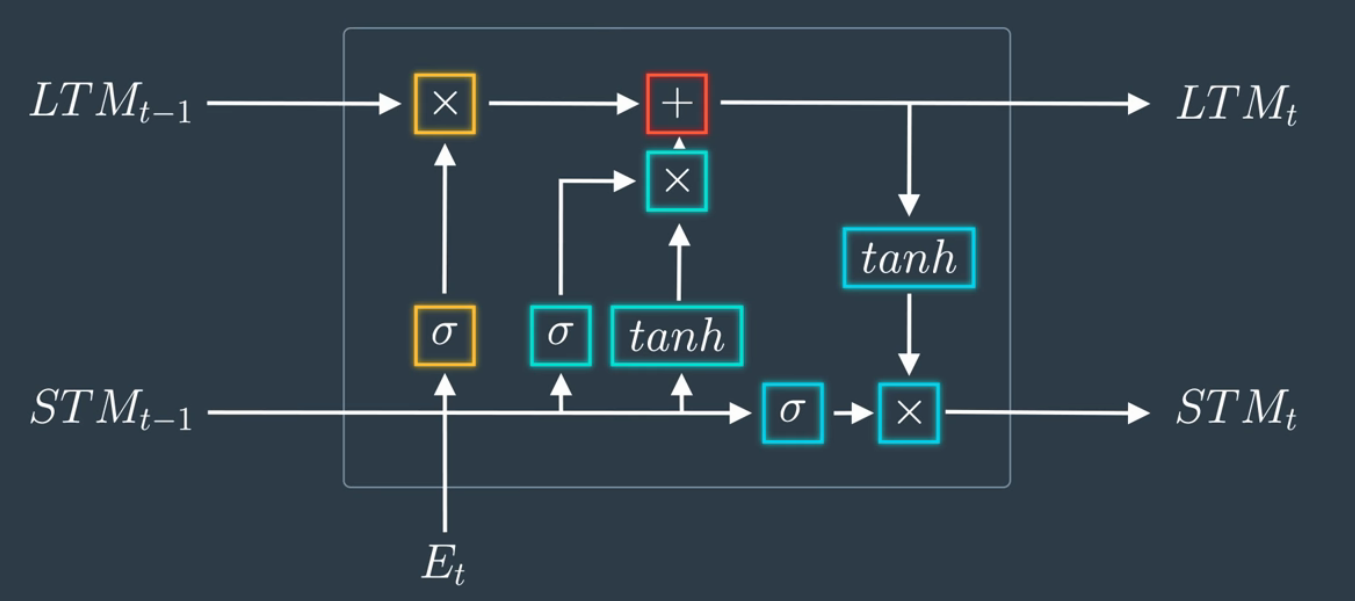
\includegraphics[width=0.65\textwidth,height=0.65\textheight,keepaspectratio]{images/lstm_node.png}
    \captionsetup{justification=centering}
    \caption{Operations behind a LSTM node}
    \label{fig:f10}
\end{figure}

Let's start with the explanation of each gate in the LSTM. \textbf{The learn gate} by taking the short term memory and the event and it joins it. Additionally, it takes the short term memory and the event and it combines them and then it ignores a bit of it keeping the important part of it. Mathematically, it takes the short term memory \(STM_{t-1}\) and the event \(E_t\) and it combines them by putting them through a linear function which consists of joining the vectors multiplying by a matrix adding a bias and finally squishing the result with a tanh activation function Eq. \eqref{eq:4}.

\begin{equation}
N_t =  tanh(W_n[STM_{t-1}, E_t] + b_n)
\label{eq:5}
\end{equation}

To ignore information, an ignore factor \(i_t\) is introduces. This factor i actually a vector but it multiplies element wise. To calculate this vector previous information of the short term memory and the eventt are used. The Eq. \eqref{eq:6} describes the mathematical equation to compute this factor and the Fig. \ref{fig:f13} presents the learn gate pipeline.

\begin{equation}
i_t =  \sigma(W_i[STM_{t-1}, E_t] + b_i)
\label{eq:6}
\end{equation}

\begin{figure}[ht]
    \centering
    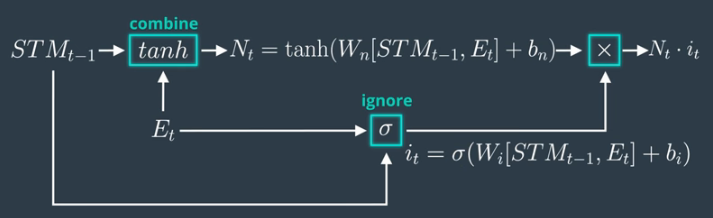
\includegraphics[width=0.65\textwidth,height=0.65\textheight,keepaspectratio]{images/learn_gate.png}
    \captionsetup{justification=centering}
    \caption{The learn gate}
    \label{fig:f13}
\end{figure}



The \textbf{forget gate} takes a long term memory and it decides what parts to keep and to forget Fig. \ref{fig:f11}. Mathematically, The long-term memory (LTM) from \(t-1\) comes in and it gets multiplied by a Forget Factor \(ft\) Eq. \eqref{eq:2}. To calculate \(ft\) the short term memory STM and the event information are used as shown by Eq. \eqref{eq:3}.

\begin{figure}[ht]
    \centering
    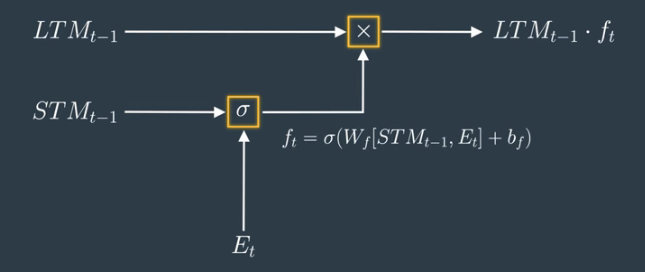
\includegraphics[width=0.65\textwidth,height=0.65\textheight,keepaspectratio]{images/forget_gate.png}
    \captionsetup{justification=centering}
    \caption{The forget gate}
    \label{fig:f11}
\end{figure}


\begin{equation}
LTM_{t-1} * ft
\label{eq:2}
\end{equation}


\begin{equation}
ft = \sigma(W_f[STM_{t-1}, E_t] + b_f)
\label{eq:3}
\end{equation}

\textbf{The remember gate} is the simplest. It takes the long-term memory coming out of the Forget Gate and the short-term memory coming out of the Learn Gate and simply combines them together Eq. \eqref{eq:4} (adding them) Fig. \ref{fig:f12}. The output of this gate is the new long term memory.


\begin{figure}[ht]
    \centering
    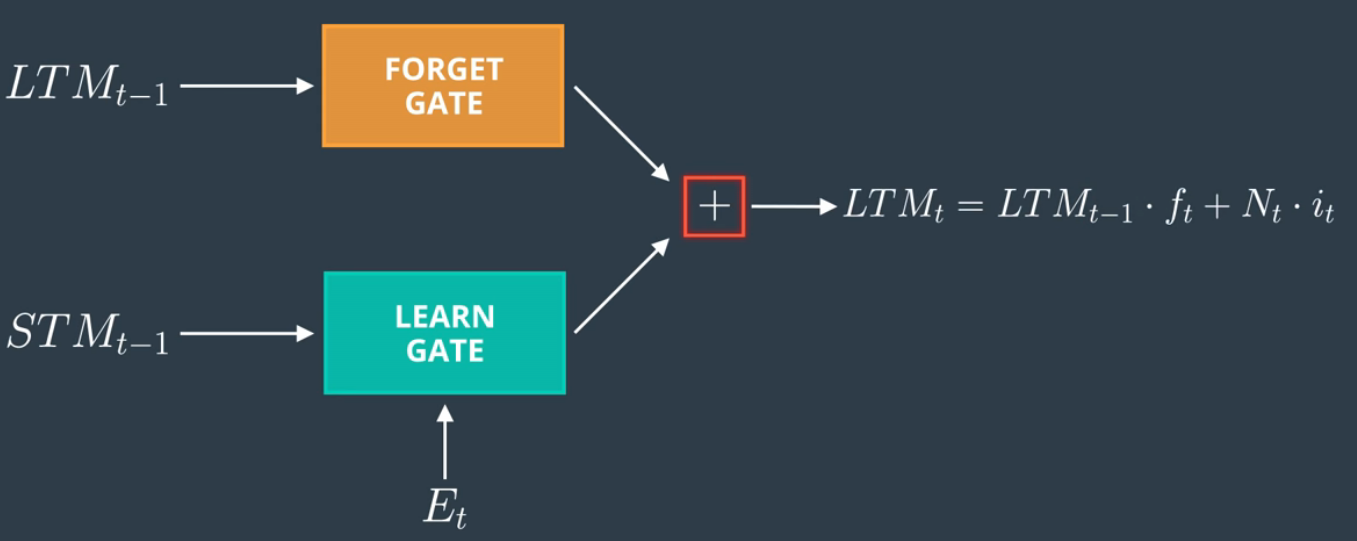
\includegraphics[width=0.65\textwidth,height=0.65\textheight,keepaspectratio]{images/remember_gate.png}
    \captionsetup{justification=centering}
    \caption{The remember gate}
    \label{fig:f12}
\end{figure}

\begin{equation}
LTM_t = LTM_{t-1} * ft + N_t * i_t
\label{eq:4}
\end{equation}

Finally, \textbf{the use gate} uses the long term memory that cames out of the forget gate and the short term memory that cames out of the learned gate, to come up with a new short term memory and an output. Mathematically, it applies

a small neural network on the output of the forget gate using the tanh activation function (Eq. \eqref{eq:7}) and it applies another small neural network on the short term memory and the events using the sigmoid activation function (Eq. \eqref{eq:8}). As a final step, it multiplies these two in order to get the new output Eq. \eqref{eq:9}. The output also worth of the new short term memory Fig. \ref{fig:f14}.

\begin{equation}
U_t = tanh(W_u LTM_{t-1} * f_t + b_u) 
\label{eq:7}
\end{equation}

\begin{equation}
V_t = \sigma(W_v[STM_{t-1}, E_t] + b_v)
\label{eq:8}
\end{equation}

\begin{equation}
STM_t = U_t * V_t
\label{eq:9}
\end{equation}


\begin{figure}[ht]
    \centering
    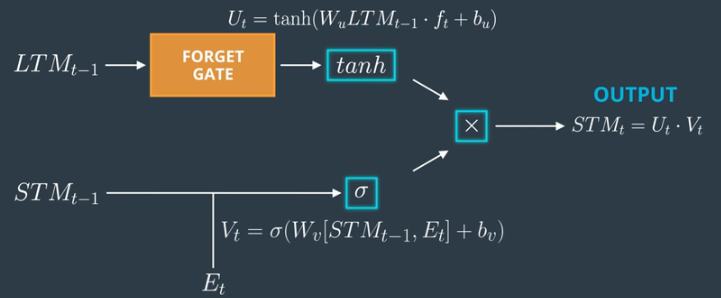
\includegraphics[width=0.65\textwidth,height=0.65\textheight,keepaspectratio]{images/use_gate.png}
    \captionsetup{justification=centering}
    \caption{The use gate}
    \label{fig:f14}
\end{figure}

\printbibliography


\end{document}

